\documentclass[a4paper,11pt,twocolumn]{article}
\usepackage[top=1.2in, bottom=1in, left=1.4in, right=1.4in]{geometry}
\usepackage{graphicx}
\usepackage{tabularx}
\usepackage{listings}
\usepackage{hyperref}
\lstset{
breaklines=true
}

\title{Firewall For Preventing Anonymous Proxy Usage\\ {\normalsize CS4099 Project\\Midterm Report}}
\author{Anant Kandikuppa, Mahesh Sreekumar Rajasree, Sri Harsha Vipparti\\Guided By: Sumesh T.A}
\begin{document}
\maketitle
\section{Introduction}
An anonymous proxy is a tool that attempts to make activity on the Internet untraceable. It can be used to prevent identity theft, or to protect search histories from public disclosure. On the other hand, it can also allow users to violate network policies of an organisation by bypassing existing security systems. Hence there is a need for proxy usage to be monitored within an organisation.\\
There are two kinds of anonymous proxies - one that is specific to a particular protocol say, HTTP, and the other being protocol independent.\\
The advantage of a protocol specific anonymizer is that no extra software is needed. The operation occurs in this manner: A connection is made by the user to the anonymizer. Commands to the anonymizer are included inside a typical message. The anonymizer then makes a connection to the resource specified by the inbound command and relays the message with the command stripped out.\\
Protocol independence can be achieved by creating a tunnel to an anonymizer. The technology to do so varies. Protocols used by anonymizer services may include SOCKS, PPTP, or OpenVPN.\\
Most of the traffic routed to such proxy servers originates from web browsers and thus, controlling access to HTTP/HTTPS proxies is a major concern. VPNs are used in geographically separated offices to share information securely, but the software supporting this service may be reconfigured to connect to rogue VPN providers and the malicious user can proxy his web activity through the VPN providers' servers. Therefore, we limit the scope of the discussion to HTTP/HTTPS proxies and VPNs only. 
\section{Problem Statement}
The problem is to prevent anonymous proxy usage within an organisation’s network. This is achieved by a browser extension working along with a backend component that captures all packets, identifies packets originating from browsers and blocks packets routed towards anonymous proxies.
\section{Literature Survey }
 A mechanism to detect commonly used proxies is given by Brozycki in \cite{brozyckidetecting}.The Request For Comments for the IPSec protocol are presented in \cite{RFC4301}. Methods to attack VPN's are discussed in \cite{adrianimperfect}
\section{Work Done in the previous semester}
From the literature survey, it became obvious to us that current methods that block  URLs using manual blacklisting cannot provide a reliable solution. Further with the widespread usage of strong encryption in network traffic, it is not possible to efficiently extract useful information from the communications. Hence we decided to attack this problem by observing packet headers.To study the differences in packet headers (with and without proxy usage), packets were captured using two tools -\textbf{ mitmproxy} and \textbf{Wireshark}.

\subsection{Packet Analysis}

\subsubsection{Web Proxy}
To capture traffic generated by web proxies, \textbf{mitmproxy} was used.
\textbf{mitmproxy} is an interactive, SSL-capable man-in-the-middle proxy for HTTP/HTTPS. It allows us to intercept HTTP/HTTPS requests and responses and modify them. Using this tool, the responses of the top ten free web proxy services were compared with those of the actual server. The following observations were made :
\begin{enumerate}
\item The following HTTP header fields were found to be different
\begin{itemize}
\item Server
\item Set Cookie
\item Keep-Alive
\item Content-Length (except for a few cases)
\end{itemize}
\item The following changes were observed in the packet body
\begin{itemize}
\item The GET/POST form variables contained URLs (user-requested URLs)
\item Additional header and footer were added to the page
\item All the links were modified to hide the actual server hostname
\item In some cases, the page contents were encrypted and were decrypted in the browser using JavaScript.
\end{itemize}
\end{enumerate}

From the above observations, the following conclusions were made:
\begin{itemize}
\item The Server, Set Cookie, Keep-Alive, Content-Length fields in the HTTP response headers would remain unchanged if proxies were not used
\item A URL in the GET/POST form data shows that there might be a possibility that the receiver is a proxy server.
\item Majority of the response body obtained through a proxy server would match the original response.
\end{itemize}

\subsubsection{Virtual Private Networks (VPNs)}
The previous observations will not be possible in the case of usage of VPNs. This is because the application and transport layer contents are encrypted. Attacking the cryptography behind VPNs is not feasible with our limited resources, as shown in \cite{adrianimperfect}. Thus, the only usable information that can be extracted is the network layer header which includes the source and destination IP address.\\
For understanding VPN traffic, packets were analyzed using \textbf{Wireshark}. \textbf{Wireshark} is a free network protocol analyzer that allows us to capture and filter packets. Using this tool, we observed that:
\begin{itemize}
\item Destination IP is different from the IP of the original host
\item Contents of other layers are obfuscated
\end{itemize}

From these observations, we can conclude that usage of VPNs can be identified by differences in the destination IP addresses.

\subsection{Design}
Based on the conclusions drawn from the analysis of web proxies and VPNs, we found that the solution would have to work at both the application and the network layer to work around the problem of encryption.\\
The solution that we came up with involves a browser extension and a backend component running on the client's system. \\The browser extension allows us to intercept and freely alter HTTP/HTTPS requests and responses. This allows us to avoid decrypting SSL traffic and obtain form data easily. \\The backend component captures all the packets at the network layer and allows us to obtain destination IP addresses.\\
These components work together to prevent the usage of both web proxies and VPNs.\\

\begin{figure*}[htp]
\centering
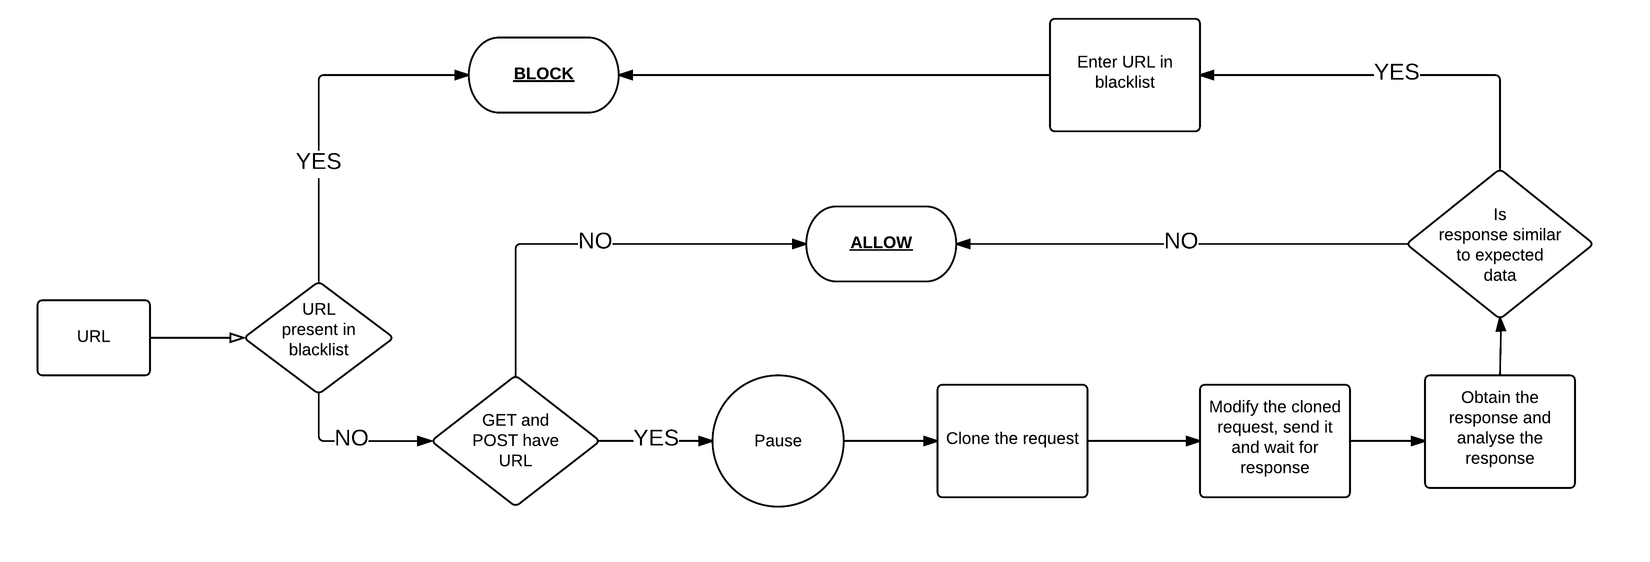
\includegraphics[scale=1.00]{rsz_proxy_avoiding_firewall_-_new_page.png}
\caption{Detecting and Blocking Web Proxies}
\label{}
\end{figure*}
\subsubsection{Blocking Web Proxies}
The browser extension is primarily used to detect and block web proxies. \\The extension maintains a blacklist of blocked URLs that is populated over time.
The following steps are performed in the browser extension in order to detect and block web proxy usage:
\begin{enumerate}
\item Obtain URL from HTTP/HTTPS request.
\item If URL is already present in the blacklist, block the request
\item Else, pause the current request
\item Clone the paused request
\item Search for URL-like patterns in the GET/POST request data of the cloned request and replace it with a \textbf{reference URL}. The  \textbf{reference URL} is a URL of an HTML page which contains a large prime number, to uniquely identify the page, and is hosted by us.
\item Send the modified request and wait for response
\item If the response contains the large prime number, then URL is a proxy URL and can be blacklisted
\item Otherwise, the original request can be allowed to proceed normally
\end{enumerate}
\begin{figure*}[htp]
\centering
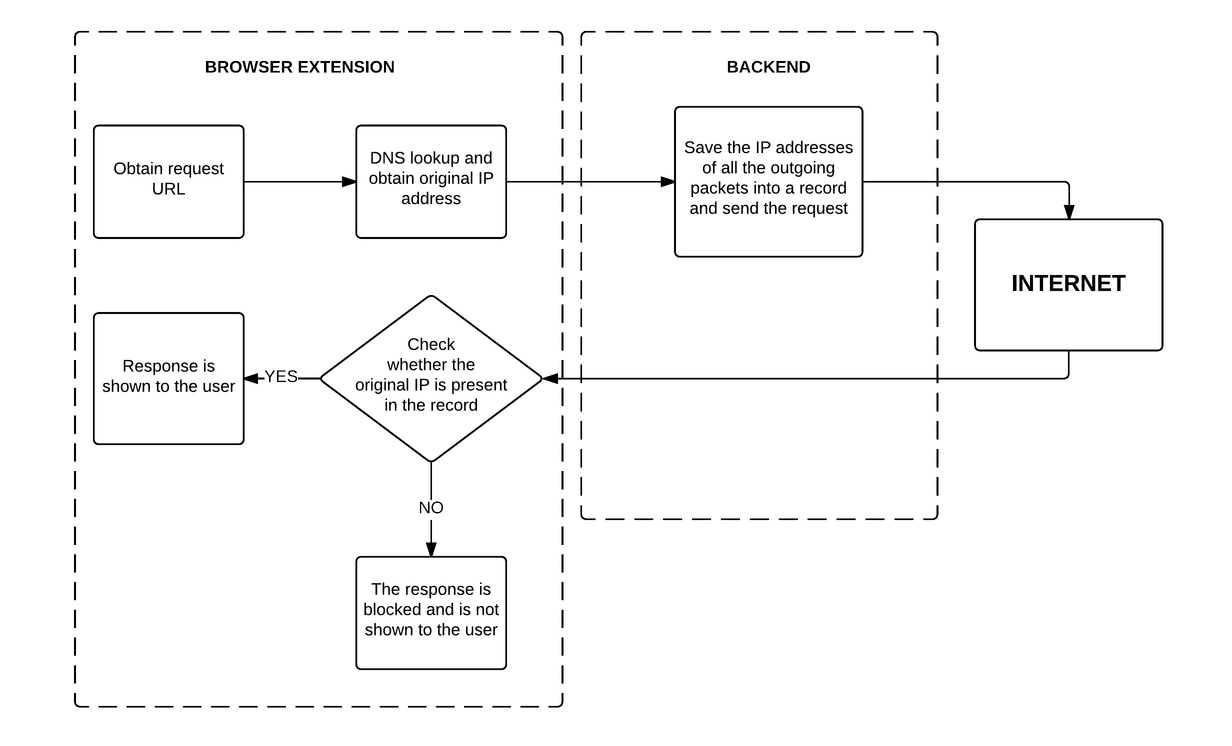
\includegraphics[scale=1.00]{rsz_vpn_flow_diagram_-_new_page.png}
\caption{Detecting and Blocking VPNs}
\label{}
\end{figure*}
\subsubsection{Blocking Virtual Private Networks}
The above method works for the case of web proxies, but in the case of VPNs, a different approach is needed.\\
We propose the following approach to detect and block VPN usage:
\begin{enumerate}
\item Obtain the URL of a HTTP/HTTPS request
\item Using the URL, obtain the IP address \begin{math}IP_{original}\end{math} via a DNS lookup.
\item At the backend, all the IP addresses of the outgoing packets are stored in a record
\item On receiving the response, the extension checks whether the original IP, \begin{math}IP_{original}\end{math} is present in the records
\item If it is not present, that implies that the packets corresponding to this request, were routed through a different path. Such a response is blocked and not shown to the user.
\item Otherwise, the response is allowed to be displayed by the browser
\end{enumerate}

For allowing access to legitimate VPNs, a whitelist can be maintained to specify the IP addresses of the VPN servers which can be legitimately accessed from within the organization.

\subsubsection{Collaborative Blacklisting}
Our solution has a feature that allows multiple clients to collaborate to build better blacklists by sharing their blacklists. Each client periodically synchronizes its blacklist with the blacklist present in the central server. The blacklist in the server is also updated as and when new entries are inserted in any of the clients.

\subsubsection{Reference URL} \label{url}
As mentioned before, the reference URL is a URL that points to an HTML page containing a large prime number.\\
Given a URL, a web proxy returns the resource present at the particular URL. To check whether a particular site is a web proxy, we are creating a new request with this reference URL in place of the URL present in the form data. In case the site is a web proxy, the response would contain the HTML page addressed by our reference URL. But, if the site is not a web proxy, it might return a different response. In order to distinguish between these responses, we are using a very large prime number \begin{math}P\end{math}, say about 100 digits long. Here, \begin{math}P\end{math} ensures that the possibility of getting false positives is very rare, as it would not be expected to be seen in any other webpage.\\
As the webpage is hosted by us, we can determine the expected values for the various HTTP header fields and these can be easily verified by the browser extension.
\section{Work Done in the current semester}
 The implementation was started by handling web proxies. The initial design included a browser extension that would block proxy websites. The following problems were encountered while implementing our previous design :
 \begin{itemize}
 	\item There was a lack of API support available for modifying the HTTP request body and for cloning the requests.
 	\item The extension supports only asynchronous HTTP calls, which are not desirable for our use case. In order to block HTTP requests, support for synchronous HTTP calls was required.
 \end{itemize}
\textbf{mitmproxy} provides all the desired features plus the added benefit of using it as a transparent proxy which allows our application to block HTTP/S requests originating from any application in our system, rather than restricting it to only web browsers.

The design of our application was therefore modified, replacing the extension with an inline script running within mitmproxy.

\subsection{Implementation Details}
\subsubsection{GET/POST Requests} \label{requests}
In order to filter out suspicious requests, our application searches for url like patterns in the GET/POST request data. The following regular expression was used to search for such patterns -
\begin{verbatim}
(((https?:\/\/)?(www\.)?)?
([a-zA-Z0-9@:%._\+~#=]{2,256}\
.[a-z]{2,6})\b
([-a-zA-Z0-9@:%_\+.~#?&//=]*))
\end{verbatim}

When a suspicious POST request is made to the proxy server, it returns a redirect URL. The resource at this URL is then fetched by our application. In order to be able to fetch the resource, the GET request should bear a cookie value that the proxy server expects. The application copies and updates the cookie fields in the GET request depending on the previous communication with proxy server.

\subsubsection{Blacklisting}
The application maintains a blacklist of URLs to block proxy sites that were encountered in the past in a SQLite database. The peculiarity of our problem is that the vast majority of the URLs encountered would be legitimate and queries to the database in such cases would slow down such traffic to a large extent. This calls for an additional data structure that allows for fast lookups and has low space requirements. One such data structure is a \textbf{Bloom Filter}.\\

Bloom filter is a probabilistic data structure to determine if an element is either definitely absent from the set or maybe present in the set. Bloom filters have a strong space advantage over other data structures for representing sets, such as self-balancing binary search trees, tries, hash tables, or simple arrays or linked lists of the entries.\\

	An empty Bloom filter is a bit array of m bits, all set to 0. It also has k different hash functions defined, each of which maps some set element to one of the m array positions with a uniform random distribution. To add an element, it should be fed to each of the k hash functions to get k array positions which are set to 1. To query for an element, the element is fed to each of the k hash functions to get k array positions. If any of the bits at these positions is 0, the element is definitely not in the set and if all are 1, then either the element is in the set, or the bits have by chance been set to 1 during the insertion of other elements, resulting in a false positive.\\

	Given a Bloom filter with m bits and k hash functions, both insertions and membership testing are O(k).The false positive error rate is approximately $ (1-e^{-kn/m})^{k} $  where $k =$ number of hash functions, $n =$ number of elements already inserted into the filter and $m =$ number of bits of the filter.\\

	For our project, we are using the pybloomfiltermmap library for Python. The hash functions used in python-bloomfilter are either sha512, sha384, sha256, sha1 or md5 (depending on the size of the bloom filter that we are using and the error rate) and are independent and uniformly distributed.The application in our case uses a constant space bloom filter having 10000000 bits and 0.01 false positive error rate.

\subsubsection{Reference site}
As described in \ref{url}, the reference HTML page which contains the random 100 digit prime number is currently hosted at \url{athena.nitc.ac.in/anant_b120519cs/refURL}. 

\subsubsection{Encrypted Pages} \label{enc_page}
Some proxy sites offer the option of returning proxied pages in an encrypted form. The pages returned by the proxy contain JavaScript code that decrypts the contents when executed in a web browser. This form of encrpytion is able to fool our application as our reference prime would not be present as is in the response text. In order to get around this problem, we need to be able to execute JavaScript code within our application itself, and then look for the reference prime in the page. We have planned to accomplish this using PhantomJS and Selenium, which allow us to test web applications from within our Python script. Initial attempts at blocking encrypted pages using this technique haven't worked out as we are facing a few problems with cookies as explained in \ref{requests}

\subsection{Results} \label{result}
\subsubsection{Effectiveness}
To test the effectiveness of our solution, we tested our application against the following proxy sites :
\begin{itemize}
\item{hide.me}
\item{hidester.com}
\item{proxysite.com}
\item{filterbypass.me}
\item{unblockmyweb.com}
\end{itemize}

\begin{table*}[t]
\centering
\caption{Effectiveness of the application} \label{effect}
	\begin{tabular}{|c|c|c|c|}
	\hline
	Proxy Site&None&Encrypt URL&Encrypt Page \\
	\hline
	hide.me & Blocked & Blocked & Allowed\\
	\hline
	hidester.com & N.A & N.A & Allowed\\
	\hline
	proxysite.com &  N.A & Blocked & N.A\\
	\hline
	filterbypass.me & Blocked & Blocked & Allowed\\
	\hline
	unblockmywed.com &N.A & Blocked  & N.A\\
	\hline
	\end{tabular}
\end{table*}
\begin{table*}[t] 
\centering
\caption{Efficiency (page load time in s)} \label{efficiency}
	\begin{tabular}{|c|c|c|c|}
	\hline
	Cases&Baseline&Fresh Request&Repeated Request \\
	\hline
	Case 1& 7.1 & 10.16 & N.A\\
	\hline
	Case 2 & 5.0 & 10.42 & N.A\\
	\hline
	Case 3 &  N.A & 6.2 & 2.5\\
	\hline
	\end{tabular}
\end{table*}
As seen in Table \ref{effect} the application is able to block proxy sites which do not encrypt the requested page as in the case of hidester.me, which encrypts the requested pages by default. hide.me and filterbypass.me offer users the option to do the same, but the option is not enabled by default. In all other cases, the proxy sites are blocked. 

\subsubsection{Efficiency}
For analysing the efficiency of our solution, we considered the following cases:
\begin{enumerate}
	\item{Normal request without any URL like patterns in the form data.}
	\item{Request with URL like patterns but not a proxy request.}
	\item{Request with URL like patterns to a proxy server.}
\end{enumerate}

The page load times seen in Table \ref{efficiency} were observed in firefox browser with an empty cache.

\section{Future Work and Conclusions}
From the results shown in \ref{result}, we can conclude that the solution that we present is effective and further work is required to improve its efficiency as well as functionality. \\

The remaining work to be done is as follows:

\subsection{Handling Encrypted Pages}
The tools required for implementing this feature have been identified in \ref{enc_page}. We are currently facing a problem with setting cookies in the GET request as discussed in \ref{requests}.

\subsection{Collaborative Blacklisting}
For implementing collaborative blacklisting, we need to find an efficient algorithm that minimizes network communication and ensures coherence across multiple clients. Each client currently maintains a database and a bloomfilter to store the blacklist. Both of these would have to be updated to ensure sites previously identified as proxy sites are blocked immediately in the future. 
\subsection{Blocking VPNs}
The tools required for blocking VPNs as per our earlier design have been studied. The implementation would begin after the work on web proxies is completed.

\subsection{Improving Efficiency}
In its current form, the application has a considerable effect on the page load time. One of the sources of this delay might be the fact that we are running our scripts within the mitmproxy application. Running our script as a standalone application using the libraries provided by mitmproxy, might improve the page load time. 
\bibliographystyle{plain}
\bibliography{ref}
\end{document}

